% 1.1.ConventionMethod.tex
%	Last update: 2019/07/24 F.Kanehori
%\newpage
\subsection{従来の方法}
\label{subsec:ConventionalMethod}

\noindent
GitHubからSpringheadをダウンロードすると、
\SprLib をビルドするためのソリューションファイル
およびプロジェクトファイルがその中に含まれています。

\medskip
\ifLwarp
\Vskip{-.8\baselineskip}
\begin{narrow}[15pt]
	\begin{figure}[h]
	    \begin{center}
	    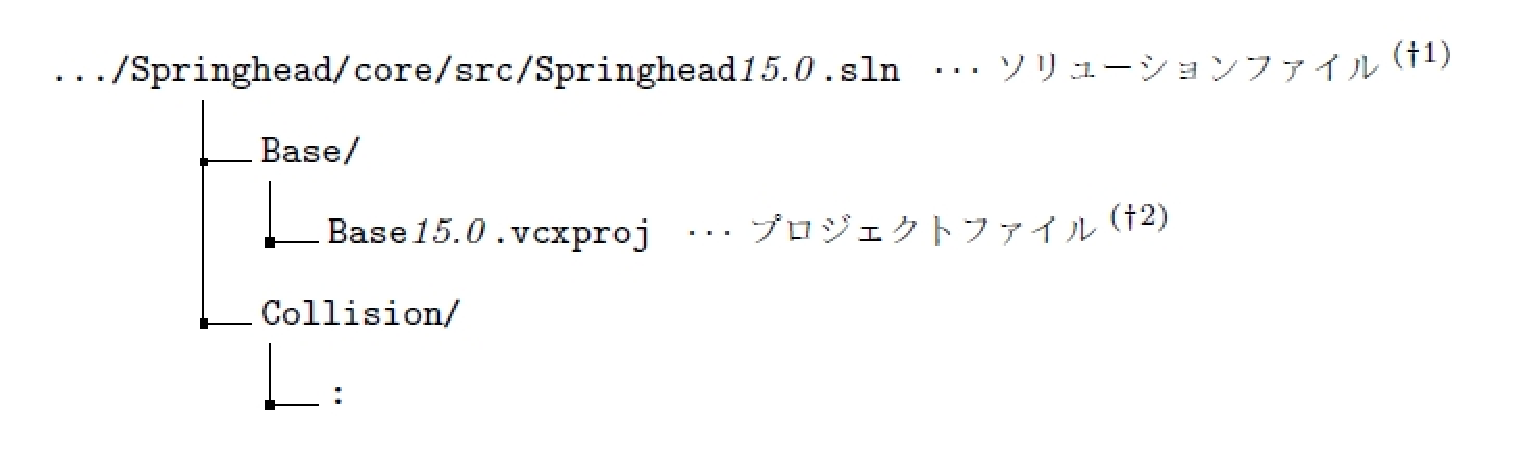
\includegraphics[width=.9\textwidth]{fig/DownloadTree.eps}
	    \end{center}
	    \label{fig:DownloadTree}
	\end{figure}
\end{narrow}
\Vskip{-.8\baselineskip}
\else
\begin{narrow}
    \begin{narrow}[20pt]\begin{minipage}{\textwidth}
	{\footnotesize{\dirtree{%
		.1 \hspace{-10mm}.../Springhead/core/src/Springhead\it{15.0}.sln
			\Anno{\SolutionFile}.
		.2 Base/.
		.3 Base\it{15.0}.vcxproj
			\Anno{\ProjectFile}.
		.2 Collision/.
		.3 :.
	}}}
	\medskip
  \end{minipage}\end{narrow}
\end{narrow}
\fi

\noindent
上記の\SolutionFile を実行すれば\SprLib を生成することができ、
アプリケーションプログラム用のソリューションファイルに
上記の\ProjectFile を\KQuote{既存のプロジェクト}として追加すれば、
アプリケーションと\SprLib の開発が同時に行えました。

後者の場合は、\ProjectFile は直接共有されることになります。
このため、複数のソリューションファイルを同時に開き、あるアプリケーションで
\ProjectFile に変更が及ぶような修正(ソースファイルの追加・削除)を実施しても、
その変更が他のアプリケーションにも直ちに反映されました
(プロジェクトが環境外で変更された旨のダイアログが出ます)。

\medskip
\noindent
この方法はうまく機能していますが、強いて言えば次の点が難点として挙げられます。

\Vskip{-.5\baselineskip}
\begin{itemize}
  \item	Visual Studioのバージョンが変わる度に、
	ソリューションファイルとプロジェクトファイルを作り直す必要がある。
  \item	Windows以外のプラットフォームに対しては、
	Makefileなどを別途作成する必要がある。
\end{itemize}

% end 1.1.ConventionMethod.tex
